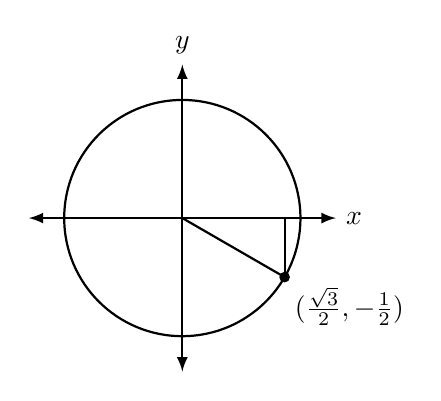
\begin{tikzpicture}[>=latex,scale=1.5,thick]
\draw [<->](-1.3,0)--(1.3,0) node [right] {$x$};
\draw [<->] (0,-1.3) -- (0,1.3) node [above] {$y$};
\draw (0,0) circle (1);
\draw [fill= black] (.866,-.5) circle (1pt);
	\draw (0,0) -- (.866,-.5) node [below right] {$(\frac{\sqrt{3}}{2}, -\frac{1}{2})$};
\draw (.866,-.5) -- (.866,0);
\end{tikzpicture}

